\section{Influence de l'inclinaison de l'arme (Cant)}

\subsection{Introduction}

Lorsqu'une arme est réglée (\textit{zérotée}) pour une distance donnée, l'axe du canon n'est pas parfaitement aligné avec la ligne de visée. Afin de compenser la chute du projectile sous l'effet de la gravité, le canon est orienté selon un faible angle vers le haut.

Tant que l'arme reste verticale, cette compensation agit uniquement dans le plan vertical. En revanche, lorsque l'arme est inclinée autour de son axe longitudinal (\textit{cant}), une partie de cette compensation est transférée dans le plan horizontal.

Ce phénomène provoque simultanément :

\begin{itemize}
\item une erreur verticale ;
\item une erreur latérale ;
\item une rotation du plan de trajectoire.
\end{itemize}

\subsection{Arme tenue normalement}

Lorsque l'arme est maintenue verticale, la hauteur de visée $h$ est située directement au-dessus de l'axe du canon.

\begin{figure}[H]
\centering
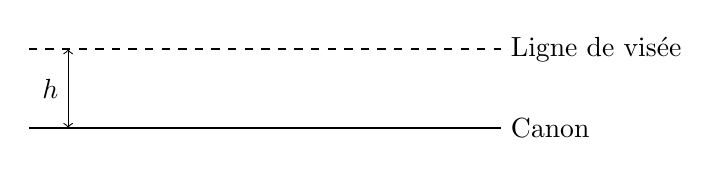
\begin{tikzpicture}[scale=1]

\draw[thick] (0,0) -- (6,0);
\draw[thick,dashed] (0,1) -- (6,1);

\draw[<->] (0.5,0) -- (0.5,1);
\node[left] at (0.5,0.5) {$h$};

\node[right] at (6,0) {Canon};
\node[right] at (6,1) {Ligne de visée};

\end{tikzpicture}
\caption{Configuration normale de tir}
\end{figure}

Le projectile coupe alors la ligne de visée à la distance de réglage.

\subsection{Arme inclinée de 90\textdegree}

Après une rotation de 90\textdegree\ vers la droite (sens horaire), la hauteur de visée se retrouve entièrement sur le côté.

\begin{figure}[H]
\centering
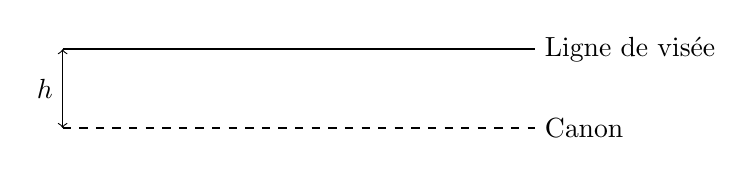
\begin{tikzpicture}[scale=1]

\draw[thick] (0,0) -- (6,0);
\draw[thick,dashed] (0,-1) -- (6,-1);

\draw[<->] (0,-1) -- (0,0);
\node[left] at (0,-0.5) {$h$};

\node[right] at (6,0) {Ligne de visée};
\node[right] at (6,-1) {Canon};

\end{tikzpicture}
\caption{Rotation de 90\textdegree\ vers la droite (sens horaire)}
\end{figure}

Pour maintenir le réticule sur la cible, le tireur doit réorienter légèrement l'arme. La trajectoire est alors déplacée :

\begin{itemize}
\item vers la gauche ;
\item vers le bas.
\end{itemize}

Une inclinaison de 90\textdegree\ produit ainsi l'erreur maximale.

\subsection{Décomposition géométrique}

Pour une inclinaison $\phi$, la hauteur de visée se décompose selon deux composantes :

\begin{align}
h_v &= h \cos \phi \
h_h &= h \sin \phi
\end{align}

où :

\begin{itemize}
\item $h_v$ est la composante verticale ;
\item $h_h$ est la composante horizontale.
\end{itemize}

L'erreur latérale à la distance de réglage est donnée par :

\begin{equation}
E_{lat}=h \sin\phi
\end{equation}

L'erreur verticale vaut :

\begin{equation}
E_{vert}=h\left(1-\cos\phi\right)
\end{equation}

\subsection{Exemple numérique}

Considérons :

\begin{itemize}
\item une hauteur de visée de 5 cm ;
\item un réglage à 100 m.
\end{itemize}

Les erreurs géométriques obtenues sont résumées dans le tableau \ref{tab:cant_error}.

\begin{table}[H]
\centering
\caption{Erreur induite par l'inclinaison de l'arme}
\label{tab:cant_error}
\begin{tabular}{ccc}
\toprule
Inclinaison & Erreur latérale & Erreur verticale \\
\midrule
5\textdegree  & 0.44 cm & 0.02 cm \\
15\textdegree & 1.29 cm & 0.17 cm \\
30\textdegree & 2.50 cm & 0.67 cm \\
45\textdegree & 3.54 cm & 1.46 cm \\
90\textdegree & 5.00 cm & 5.00 cm \\
\bottomrule
\end{tabular}
\end{table}

\subsection{Visualisation des impacts}

\begin{figure}[H]
\centering
\begin{tikzpicture}[scale=1]

\draw[->] (-6,0) -- (6,0);
\draw[->] (0,-6) -- (0,2);

\filldraw (0,0) circle (2pt);
\node[above right] at (0,0) {0\textdegree};

\filldraw (-0.44,-0.02) circle (2pt);
\node[left] at (-0.44,-0.02) {5\textdegree};

\filldraw (-1.29,-0.17) circle (2pt);
\node[left] at (-1.29,-0.17) {15\textdegree};

\filldraw (-2.50,-0.67) circle (2pt);
\node[left] at (-2.50,-0.67) {30\textdegree};

\filldraw (-3.54,-1.46) circle (2pt);
\node[left] at (-3.54,-1.46) {45\textdegree};

\filldraw (-5,-5) circle (2pt);
\node[left] at (-5,-5) {90\textdegree};

\node[below] at (0,-6) {Bas};
\node[left] at (-6,0) {Gauche};

\end{tikzpicture}
\caption{Déplacement du point d'impact pour une inclinaison vers la droite (sens horaire)}
\end{figure}

\subsection{Conséquences en tir longue distance}

À courte distance, l'erreur est principalement liée à la hauteur de visée. En revanche, à longue distance, l'inclinaison agit également sur les corrections de chute appliquées par le système de visée.

Si la correction balistique représente plusieurs mètres à la distance d'engagement, une faible inclinaison peut engendrer une dérive latérale importante.

Par exemple, pour une correction verticale de 5 m :

\begin{equation}
D = 5 \sin(5^\circ)
\end{equation}

ce qui représente environ :

\begin{equation}
D \approx 0.44,m
\end{equation}

soit près de 44 cm de dérive latérale.

\subsection{Conclusion}

L'inclinaison de l'arme transforme une partie de la correction verticale en correction horizontale. Plus la distance augmente, plus cette erreur devient significative.

Pour cette raison, les systèmes destinés au tir de précision sont fréquemment équipés d'un niveau à bulle permettant de vérifier la verticalité de l'arme avant le tir.

\subsection{Remarque sur le sens d'inclinaison}

Les exemples présentés dans cette annexe correspondent à une inclinaison vers la droite (sens horaire). Une inclinaison vers la gauche (sens trigonométrique) produit exactement les mêmes effets, mais avec un décalage latéral de signe opposé. Ainsi, toute dérive observée vers la gauche lors d'une inclinaison vers la droite (sens horaire) devient une dérive vers la droite pour une inclinaison identique vers la gauche (sens trigonométrique).

\subsection{Cas particulier d'une rotation de 180\textdegree}

Lorsque le système est complètement retourné, la hauteur de visée se retrouve sous l'axe de lancement. La géométrie du réglage est alors inversée : l'axe de lancement est orienté légèrement sous la ligne de visée alors qu'il est normalement orienté légèrement au-dessus.

La trajectoire reste soumise à la gravité et conserve donc la même courbure dans le référentiel terrestre. En revanche, sa position relative par rapport à la ligne de visée est inversée. Le point d'impact se retrouve alors nettement plus bas que celui obtenu avec le système dans sa position normale.

Ce cas extrême constitue une illustration intéressante du fait que la gravité agit indépendamment de l'orientation du système. Ce n'est pas la trajectoire physique qui change de nature, mais le repère géométrique utilisé pour la viser et l'interpréter.

En résumé, la trajectoire du projectile ne « sait » pas que le système a été incliné ou retourné. Les effets observés proviennent uniquement de la rotation du repère de visée par rapport à la direction constante de la gravité.

Le cas d'une rotation de 180\textdegree\ constitue une expérience de pensée utile. Il montre que le réglage d'une arme repose avant tout sur la géométrie relative entre l'axe du canon et la ligne de visée. La trajectoire physique du projectile demeure soumise aux mêmes lois, indépendamment de l'orientation du système dans la main du tireur.

\begin{figure}[H]
\centering

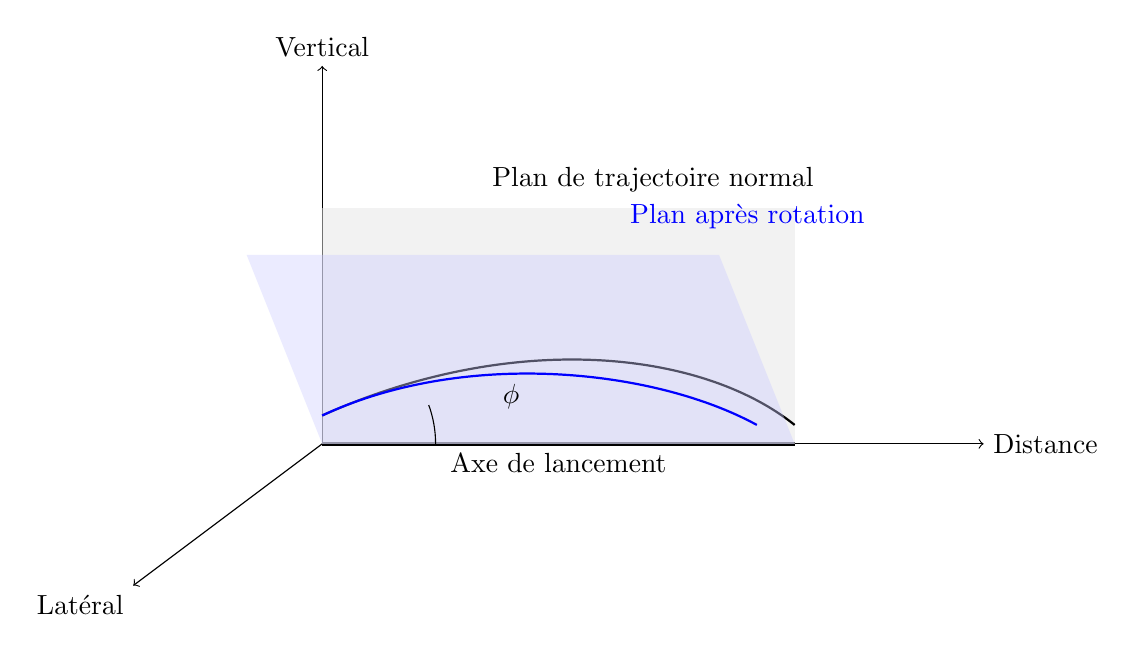
\begin{tikzpicture}[scale=1.2]

% Axes
\draw[->] (0,0) -- (7,0) node[right] {Distance};
\draw[->] (0,0) -- (0,4) node[above] {Vertical};
\draw[->] (0,0) -- (-2,-1.5) node[below left] {Latéral};

% Tube
\draw[very thick] (0,0) -- (5,0);

\node[below] at (2.5,0) {Axe de lancement};

% Plan vertical initial
\fill[gray!20,opacity=0.5]
(0,0) --
(5,0) --
(5,2.5) --
(0,2.5) -- cycle;

\node at (3.5,2.8) {Plan de trajectoire normal};

% Trajectoire normale
\draw[thick]
(0,0.3)
.. controls (2,1.2) and (4,1.0)
.. (5,0.2);

% Plan incliné
\fill[blue!20,opacity=0.4]
(0,0) --
(5,0) --
(4.2,2.0) --
(-0.8,2.0) --
cycle;

\node[blue] at (4.5,2.4)
{Plan après rotation};

% Trajectoire inclinée
\draw[blue,thick]
(0,0.3)
.. controls (1.5,1.0) and (3.5,0.8)
.. (4.6,0.2);

% Angle de rotation
\draw (1.2,0)
arc[start angle=0,end angle=20,radius=1.2];

\node at (2.0,0.5) {$\phi$};

\end{tikzpicture}

\caption{Rotation du plan de trajectoire lors de l'inclinaison de l'axe de lancement. La trajectoire reste contenue dans son plan propre, mais ce plan pivote autour de l'axe longitudinal.}
\label{fig:rotation_plan_trajectoire}

\end{figure}

